\documentclass[hyperref=unicode,presentation,10pt]{beamer}

\usepackage[absolute,overlay]{textpos}
\usepackage{array}
\usepackage{graphicx}
\usepackage{adjustbox}
\usepackage[version=4]{mhchem}
\usepackage{chemfig}
\usepackage{caption}

%dělení slov
\usepackage{ragged2e}
\let\raggedright=\RaggedRight
%konec dělení slov

\addtobeamertemplate{frametitle}{
	\let\insertframetitle\insertsubtitle}{}
\addtobeamertemplate{frametitle}{
	\let\insertframesubtitle\insertsectionhead}{}

\makeatletter
\CheckCommand*\beamer@checkframetitle{\@ifnextchar\bgroup\beamer@inlineframetitle{}}
\renewcommand*\beamer@checkframetitle{\global\let\beamer@frametitle\relax\@ifnextchar\bgroup\beamer@inlineframetitle{}}
\makeatother
\setbeamercolor{section in toc}{fg=red}
\setbeamertemplate{section in toc shaded}[default][100]

\usepackage{fontspec}
\usepackage{unicode-math}

\usepackage{polyglossia}
\setdefaultlanguage{czech}

\def\uv#1{„#1“}

\mode<presentation>{\usetheme{default}}
\usecolortheme{crane}

\setbeamertemplate{footline}[frame number]

\usepackage{tikz}
\usetikzlibrary{positioning}
\usetikzlibrary{arrows}
\usetikzlibrary{shapes.multipart}

\title[Crisis]
{NMR}

\subtitle{Nukleární Magnetická Rezonance}
\author
{\includegraphics[keepaspectratio,height=.5\textheight]{img/1H-ethylbenzen-300.png}\\
	Zdeněk Moravec, hugo@chemi.muni.cz}
\date{}

\begin{document}
\frame{\titlepage}

\section{Princip}
\frame{
	\frametitle{}
	\vfill
	\begin{columns}
		\begin{column}{.6\textwidth}
			\begin{itemize}
				\item NMR -- Nukleární Magnetická Rezonance
				\item Sledujeme absorpci radiofrekvenčního záření vzorkem, který je umístěn v silném magnetickém poli.
				\item Vzorek je nejčastěji kapalný, ale lze měřit i pevné látky a plyny.
				\item Jde o důležitou metodu v chemické a strukturní analýze.
				\item Vyžaduje silné magnetické pole, proto se nejčastěji využívá supravodivých magnetů.
			\end{itemize}
		\end{column}
		\begin{column}{.45\textwidth}
			\begin{figure}
				\includegraphics[width=.9\textwidth]{img/Bruker_500_Ultrashield_Plus.jpg}
				\caption*{NMR spektrometr 500 MHz.\footnote[frame]{Zdroj: \href{https://commons.wikimedia.org/wiki/File:Bruker_500_Ultrashield_Plus.jpg}{Steff-X/Commons}}}
			\end{figure}
		\end{column}
	\end{columns}
	\vfill
}

\section{Stručná historie}
\frame{
	\frametitle{}
	\vfill
	\begin{itemize}
	\item \textbf{1943} Nobelova cena za objev magnetického momentu protonu - Otto Stern.
	\item \textbf{1944} Nobelova cena za rezonanční metodu pro zjištění magnetických vlastností atomových jader - Isidor Isaac Rabi.
	\item \textbf{1945} \href{http://mri-q.com/uploads/3/2/7/4/3274160/blochs_first_paper_physrev.69.127.pdf}{První $^1$H NMR spektrum vody.}
	\item \textbf{1952} Nobelova cena za rozvoj metod pro přesná měření jaderného magnetismu a první NMR signál - Felix Bloch a Edward Mills Purcell.
	\item \textbf{1965} Širokopásmový $^1$H decoupling.
	\item \textbf{1991} Nobelova cena za HR-NMR, vývoj nových pulsních technik, rozvoj FT-NMR a zavedení 2D NMR technik - Richard R. Ernst.
	\item \textbf{2002} Nobelova cena za vývoj NMR technik umožňujících určení 3D struktury biomolekul - Kurt Wütthrich.
	\item \textbf{2003} Nobelova cena za vývoj MRI - Paul C. Lauterbur.
	\end{itemize}
	\vfill
}

\section{Jaderný spin}
\frame{
	\frametitle{}
	\vfill
	\begin{itemize}
	\item Atomové jádro se skládá z protonů a neutronů.
	\item Obě částice mají spin $\pm\frac{1}{2}$.
	\item Jaderný spin je roven součtu spinů všech nukleonů.
	\item V NMR jsou aktivní pouze jádra s \emph{nenulovým jaderným spinem}.
	\item Nejčastěji se využívají jádra se spinem $\frac{1}{2}$, např. $^1$H, $^{13}$C, $^{19}$F nebo $^{31}$P.
	\item Bez vlivu vnějšího magnetického pole mají všechny orientace jaderného spinu stejnou energii.
	\item Pokud ale vložíme jádro do magnetického pole, získáme systém hladin o různých energiích.
	\item Pokud na tento systém působíme radiofrekvenčním zářením, může dojít k absorpci energie a excitaci spinu na vyšší energetickou hladinu.
	\item Poté pozorujeme návrat spinu a původní hladinu a emisi absorbované energie, kterou následně snímáme.
	\end{itemize}
	\vfill
}

\frame{
	\frametitle{}
	\vfill
	\begin{figure}
		\includegraphics[height=.7\textheight]{img/NMR-levels.png}
	\end{figure}
	\vfill
}

\section{Radiofrekvenční pulsy}
\frame{
	\frametitle{}
	\vfill
	\begin{itemize}
	\item FT-NMR využívá k excitaci jaderných spinů radiofrekvenční pulsy.
	\item Ty excitují všechna měřená jádra, např. protony, najednou.
	\item Pulsy sklápí vektor magnetizace a způsobují jeho precesi.
	\item Délka pulsů se pohybuje v řádu $\mu$s.
	\item Čím je puls delší, tím je větší i sklápěcí úhel.
	\end{itemize}
	\vfill
}

\section{Chemický posun}
\frame{
	\frametitle{}
	\vfill
	\begin{itemize}
	\item Izolovaná jádra stejného izotopu budou v magnetickém poli rezonovat při stejné frekvenci.
	\item Pokud uvažujeme molekuly, je každé jádro ovlivněno také lokálními magnetickými poli, které jsou generovány vazebnými elektrony. Tím dochází ke změně rezonanční frekvence daného jádra.
	\item Změna je dána tzv. chemickým okolím pozorovaného jádra a nazývá se \emph{chemický posun}. Označuje se $\delta$ a je dán vztahem:
	\end{itemize}
	\begin{center}
	$\delta = \frac{\nu - \nu_{TMS}}{\nu}$
	\end{center}
	\begin{itemize}
	\item $\nu_{TMS}$ je rezonanční frekvence standardu, $\nu$ je rezonanční frekvence signálu.
	\item Chemický posun je bezrozměrný, jelikož se jedná o velmi malé hodnoty, udává se v ppm.
	\item Chemický posun je, na rozdíl od rezonanční frekvence, nezávislý na hodnotě vnějšího magnetického pole.
	\end{itemize}
	\vfill
}

\frame{
	\frametitle{}
	\vfill
	\begin{figure}
		\includegraphics[width=.85\textwidth]{img/NMR-fields.png}
		\caption*{Srovnání $^1$H NMR spekter ethylbenzenu na spektrometrech 60 a 300 MHz}
	\end{figure}
	\vfill
}

\section{Interakční konstanta}
\frame{
	\frametitle{}
	\vfill
	\begin{itemize}
	\item Pokud je v molekule více NMR aktivních jader, může docházet k jejich vzájemné interakci. Síla této interakce je dána hlavně počtem vazeb, které jádra oddělují.
	\item Velikost interakční konstanty je nezávislá na intenzitě magnetického pole.
	\end{itemize}
	\begin{figure}
		\includegraphics[height=.4\textheight]{img/NMR_J-coupling_trees.svg.png}
		\caption*{Příklad štěpení NMR signálu.\footnote[frame]{Zdroj: \href{https://commons.wikimedia.org/wiki/File:NMR_J-coupling_trees.svg}{Keministi/Commons}}}
	\end{figure}
	\vfill
}

\frame{
	\frametitle{}
	\vfill
	\begin{itemize}
	\item Způsob štěpení je dán počtem interagujících spinů.
	\item Pro jádra se spinem $\frac{1}{2}$ je velikost multipletu, tzn. počet signálů po štěpení a jejich vzájemná intenzita dána \textit{Pascalovým trojúhelníkem}.
	\end{itemize}
	\begin{tabular}{>{$n=}l<{$\hspace{6pt}}*{13}{c}}
	0 &&&&&&&1&&&&&&\\
	1 &&&&&&1&&1&&&&&\\
	2 &&&&&1&&2&&1&&&&\\
	3 &&&&1&&3&&3&&1&&&\\
	4 &&&1&&4&&6&&4&&1&&\\
	5 &&1&&5&&10&&10&&5&&1&\\
	6 &1&&6&&15&&20&&15&&6&&1
	\end{tabular}
	\vfill
}

\frame{
	\frametitle{}
	\vfill
	\begin{itemize}
	\item Velikost interakce se vyjadřuje pomocí interakční konstanty, která se označuje písmenem \textit{J}. Pro přesnější popis interakce se využívá
indexů, např. interakci mezi atomy vodíku v~ethanolu (přes tři vazby H-C-C-H) vyjádříme $^3J_{\textrm{HH}}$. Její velikost se udává v Hz.
	\end{itemize}
	\begin{figure}
		\includegraphics[height=.4\textheight]{img/NMR_J-coupling_trees.svg.png}
		\caption*{Příklad štěpení NMR signálu.\footnote[frame]{Zdroj: \href{https://commons.wikimedia.org/wiki/File:NMR_J-coupling_trees.svg}{Keministi/Commons}}}
	\end{figure}
	\vfill
}

\frame{
	\frametitle{}
	\vfill

	\begin{figure}
		\includegraphics[height=.75\textheight]{img/1H-ethylbenzen-300.png}
		\caption*{$^1$H NMR ethylbenzenu}
	\end{figure}
	\vfill
}

\section{Decoupling (dekaplink)}
\frame{
	\frametitle{}
	\begin{itemize}
		\item Štěpením signálů spektra je důležitou informací pro strukturní analýzu, zároveň ale zhoršuje poměr signál/šum.
		\item Pro potlačení štěpení se používá tzv. decoupling, kdy kontinuálně ozařujeme dekaplovaná jádra. Tím dojde k potlačení štěpení.
		\item Ztratíme ale informaci o kvantitativním složení vzorku, protože intenzita signálu v dekaplovaném spektru není úměrná koncentraci.
	\end{itemize}
	\begin{figure}
		\includegraphics[width=.45\textwidth]{img/APT_basic_pulse_sequence.png}
		\caption*{APT pulsní sekvence, využívá $^1$H decoupling.\footnote[frame]{Zdroj: \href{https://commons.wikimedia.org/wiki/File:APT_basic_pulse_sequence.svg}{Thypingvinen/Commons}}}
	\end{figure}
}

\frame{
	\frametitle{}
	\vfill
	\begin{figure}
		\includegraphics[height=.75\textheight]{img/13C-ethylbenzen-300.png}
		\caption*{$^{13}$C NMR ethylbenzenu s $^1$H decouplingem}
	\end{figure}
	\vfill
}

\frame{
	\frametitle{}
	\vfill
	\begin{figure}
		\includegraphics[height=.75\textheight]{img/Ethylbenzene-13C-nodec-NMR.png}
		\caption*{$^{13}$C NMR ethylbenzenu bez $^1$H decouplingu}
	\end{figure}
	\vfill
}

\section{Schéma NMR spektrometru}
\frame{
	\frametitle{}
	\vfill
	\includegraphics[keepaspectratio,width=10cm]{img/NMR-blockScheme.png}
	\vfill
}

\section{NMR magnety}
\frame{
	\frametitle{}
	\vfill
	\begin{itemize}
	\item Permanentní - do 100 MHz
	\end{itemize}
	\begin{figure}
		\includegraphics[height=.6\textheight]{img/NMR-Magritek.jpg}
		\caption*{Benchtop NMR.\footnote[frame]{Zdroj: \href{https://commons.wikimedia.org/wiki/File:Magritek_60_MHz_benchtop_NMR.jpg}{Johannes Schneider/Commons}}}
	\end{figure}
	\vfill
}

\frame{
	\frametitle{}
	\vfill
	\begin{itemize}
	\item Cryogen-free - 100-300 MHz - levný provoz
	\end{itemize}
	\begin{figure}
		\includegraphics[height=.6\textheight]{img/MR_Solutions_cryogen-free_PET-MRI_system.jpg}
		\caption*{Cryogen-free MRI magnet.\footnote[frame]{Zdroj: \href{https://commons.wikimedia.org/wiki/File:MR_Solutions\%27_cryogen-free_PET-MRI_system.jpg}{MR Solutions/Commons}}}
	\end{figure}
	\vfill
}

\frame{
	\frametitle{}
	\vfill
	\begin{itemize}
	\item Supravodivé magnety - nejběžnější v NMR
	\begin{itemize}
	\item Chlazené kapalným heliem (4-2,2 K)
	\item Magnetické pole až 23,5 T (1000 MHz)
	\end{itemize}
	\end{itemize}
	\begin{figure}
		\includegraphics[height=.5\textheight]{img/Varian-_900MHz_-_21.2_Tesla.jpg}
		\caption*{NMR spektrometr 900 MHz.\footnote[frame]{Zdroj: \href{https://commons.wikimedia.org/wiki/File:HWB-NMR_-_900MHz_-_21.2_Tesla.jpg}{MartinSaunders/Commons}}}
	\end{figure}
	\vfill
}

\section{Závislost rezonanční frekvence na síle magnetického pole}
\frame{
	\frametitle{}
	\begin{center}
		\begin{tabular}{|r@{,}l|l|r@{,}l|}
		\hline
		\multicolumn{2}{|c|}{\ce{B_0} [T]} & \ce{^1H} [MHz] & \multicolumn{2}{|c|}{\ce{^{13}C} [MHz]} \\\hline
		1 & 41 & 60 & 15 & 1 \\\hline
		2 & 35 & 100 & 25 & 15 \\\hline
		7 & 05 & 300 & 75 & 4 \\\hline
		11 & 74 & 500 & 125 & 7 \\\hline
		14 & 09 & 600 & 150 & 9 \\\hline
		16 & 44 & 700 & 176 & 05 \\\hline
		19 & 97 & 850 & 213 & 78 \\\hline
		22 & 32 & 950 & 238 & 94 \\\hline
		28 & 20 & 1200 & 318 & 59 \\\hline
		\end{tabular}
	\end{center}
}

\section{NMR sondy}
\frame{
	\frametitle{}
	\vfill
	\begin{itemize}
	\item Hlavní funkcí je excitace spinového systému a snímání odezvy.
	\item Obsahují lockovací kanál.
	\item Udržují stabilní teplotu vzorku.
	\item Často obsahují také gradientovou cívku(y) pro experimenty využívající pulsní gradienty magnetického pole.
	\item Podle konstrukce se dělí:
	\begin{itemize}
	\item Teplé sondy
	\item Kryosondy
	\item Průtočné sondy
	\item Nanosondy
	\end{itemize}
	\end{itemize}
	\vfill
}

\frame{
	\frametitle{}
	\vfill
	\begin{itemize}
	\item Sondy se dále dělí podle počtu cívek. Citlivost cívek klesá se vzdálenosti od vzorku.
	\begin{itemize}
	\item Dvoukanálové - dvě cívky
	\item Tříkanálové (triple resonance)
	\end{itemize}
	\item BB sondy mají vnitřní cívku určenou pro měření jader X a vnější pro měření $^1$H nebo $^1H$ decoupling. \emph{Inverzní sondy} mají uspořádání opačné a jsou vhodné pro snímání jader $^1$H jader, např. v 2D experimentech -- $^1$H-$^{13}$C HSQC.
	\item Sondy také dělíme sondy podle velikosti NMR kyvety, pro které jsou konstruovány, nejčastěji 5 a 10~mm.
	\end{itemize}
	\vfill
}

\frame{
	\frametitle{}
	\vfill
	\begin{columns}
		\begin{column}{.4\textwidth}
			\begin{figure}
				\includegraphics[width=.6\textheight,angle=270]{img/200MHz-Probehead.jpg}
				\caption*{NMR sonda.\footnote[frame]{Zdroj: \href{https://commons.wikimedia.org/wiki/File:19F_200MHz_Probehead.jpg}{Steff-X/Commons}}}
			\end{figure}
		\end{column}
		\begin{column}{.6\textwidth}
			\begin{figure}
				\includegraphics[width=\textwidth]{img/NMR_magnet_Julich_Germany.jpg}
				\caption*{NMR spektrometr 1.2 GHz s kryosondou.\footnote[frame]{Zdroj: \href{https://commons.wikimedia.org/wiki/File:1.2_GHz_NMR_magnet_Julich_Germany.jpg}{Adville/Commons}}}
			\end{figure}
		\end{column}
	\end{columns}
	\vfill
}

\section{Vzorky pro NMR spektroskopii}
\frame{
	\frametitle{}
	\vfill
	\begin{columns}
	\begin{column}{0.7\textwidth}
	\begin{itemize}
	\item Využívají se tenkostěnné skleněné kyvety, které se umisťují do plastových nebo keramických rotorků. Průměr kyvet je nejčastěji 3, 5 nebo 10 mm.
	\item Pro měření je nutné připravit roztok měřené látky v~deuterovaném rozpouštědle. Signál $^2$H~(D) se používá k~lockování vzorku.
	\item Vzorky reakčních směsí se často měří v~koaxiálním uspořádání, kdy se kyveta se vzorkem vloží do kyvety s deuterovaným
rozpouštědlem.
	\item Signál deuterovaného rozpouštědla lze využít i~jako standard ke kalibraci spektra.
	\end{itemize}
	\end{column}
	\begin{column}{0.3\textwidth}
		\begin{figure}
			\includegraphics[height=.67\textheight]{img/NMR-tubes.jpg}
			\caption*{Skleněné NMR kyvety.\footnote[frame]{Zdroj: \href{https://commons.wikimedia.org/wiki/File:NMR_tubes.jpg}{Edgar181/Commons}}}
		\end{figure}
	\end{column}
	\end{columns}
	\vfill
}

\section{2D NMR}
\frame{
	\frametitle{}
	\vfill
	\begin{itemize}
	\item Pro složitější molekuly už nemusí být 1D NMR spektrum čitelné.
	\item Rozlišení se dá zvýšit silnějším magnetickým polem.
	\item Lepší cestou je přechod na NMR experimenty ve dvou a více dimenzích.
	\item V dnešní době se rutinně využívá 2D a 3D NMR.
	\end{itemize}
	\begin{figure}
		\includegraphics[height=.45\textheight]{img/Noesy.jpg}
		\caption*{NOESY NMR spektrum kodeinu.\footnote[frame]{Zdroj: \href{https://commons.wikimedia.org/wiki/File:Noesy.jpg}{Acorn NMR Inc./Commons}}}
	\end{figure}
	\vfill
}

\section{NMR v pevné fázi}
\frame{
	\frametitle{}
	\vfill
	\begin{itemize}
	\item MAS NMR - Magic Angle Spinning.
	\item Vzorek je napěchován do keramického rotoru a rotuje pod úhlem 54,7$^{\circ}$ ($\cos^2\theta_m=\frac{1}{3}$, magický úhel).
	\item Rotace při rychlostech 0-130 kHz.
	\item Pro měření málo citlivých jader se využívá cross-polarizace.
	\end{itemize}
	\begin{columns}
		\begin{column}{.5\textwidth}
			\begin{figure}
				\includegraphics[height=.4\textheight]{img/MagicAngleSpinning.png}
				\caption*{Rotace pod magickým úhlem.\footnote[frame]{Zdroj: \href{https://commons.wikimedia.org/wiki/File:MagicAngleSpinning.svg}{Dtrx/Commons}}}
			\end{figure}
		\end{column}
		\begin{column}{.5\textwidth}
			\begin{figure}
				\includegraphics[height=.4\textheight]{img/MAS_rotors.jpg}
				\caption*{Rotory pro MAS NMR.\footnote[frame]{Zdroj: \href{https://commons.wikimedia.org/wiki/File:MAS_rotors.jpg}{Thomas Kress/Commons}}}
			\end{figure}
		\end{column}
	\end{columns}
	\vfill
}


\section{NMR ve slabém magnetickém poli}
\frame{
	\frametitle{}
	\vfill
	\begin{itemize}
	\item Earth's-Field NMR.
	\begin{itemize}
	\item Využívá magnetické pole Země.
	\item Lze měřit velké vzorky.
	\item Pro zlepšení S/N se využívá pre-polarizace v elektromagnetu.
	\end{itemize}
	\item Low-Field NMR.
	\item Systémy využívající permanentní magnety nebo elektromagnety.
	\end{itemize}
	\begin{figure}
		\includegraphics[height=0.37\textheight]{img/Earth_magnetic_field.png}
		\caption*{Magnetické pole Země.\footnote[frame]{Zdroj: \href{https://commons.wikimedia.org/wiki/File:Earth\%27s_magnetic_field,_schematic.svg}{Zureks/Commons}}}
	\end{figure}
	\vfill
}

\section{Využití NMR}
\frame{
	\frametitle{}
	\vfill
	\begin{itemize}
	\item Rutinní kvalitativní a kvantativní chemická analýza.
	\item Strukturní analýza.
	\item Strukturní analýza biomolekul.
	\item Studium degradačních procesů a stupně degradace, např. barviv, polymerů, atd.
	\item Studium stupně hydratace v nástěnných malbách pomocí bezkontaktní sondy.
	\end{itemize}
	\vfill
}

\section{Literatura}
\frame{
	\frametitle{}
	\vfill
	\begin{enumerate}
	\item \url{http://chem.ch.huji.ac.il/nmr/}
	\item H. Günther (2013). NMR Spectroscopy: Basic Principles, Concepts and Applications in Chemistry, ISBN 978-3527330003
	\item J. Keeler (2005). Understanding NMR Spectroscopy. ISBN 978-0-470-01786-9.
	\end{enumerate}
	\vfill
}

\end{document}